\section{Project Requirements}

This section contains the requirements created for this project, with requirement numbers for structure and clarity when referencing, as well as details for each requirement.\\

The project requirements are organized based on their specificity. At the root of the project, 5 top-level project requirements exist, each encompassing a logical component of the project.
Each of the top-level requirements is then split into parts which are more specific. Some of the parts are also split into subparts. 
The subparts, or the parts if no subparts are present, then serve as more specific requirements, guiding the creation and implementation of the software.\\

The five present top-level requirements are as follows:
\begin{itemize}
    \item \textbf{REQ1.} Search Engine
    \item \textbf{REQ2.} Backend Page Processing
    \item \textbf{REQ3.} Backend Query Processing
    \item \textbf{REQ4.} Frontend Search
    \item \textbf{REQ5.} Frontend Adding Pages
\end{itemize}

For clarity and organization, the first section of this chapter consists of a series of diagrams, intended to clarify how the top-level requirements interact with one another,
as well as how they are organized internally.

\subsection{Diagrams}

The interconnection of the top-level requirements is highlighted in the following diagram:

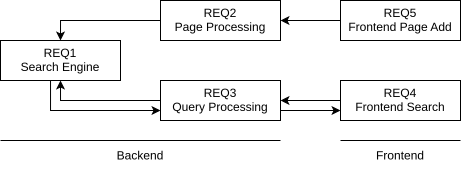
\includegraphics[width=\textwidth,keepaspectratio]{reqs.png}\\

The following diagrams represent the internal structure of the top-level requirements, the parts which they're split into and how those parts interact.\\

\textbf{REQ1:}

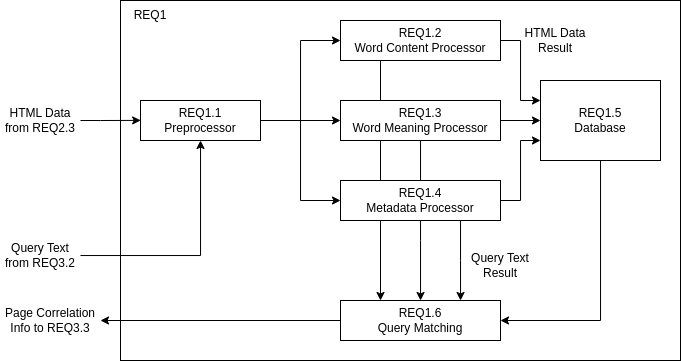
\includegraphics[width=\textwidth,keepaspectratio]{req1.png}\\

\textbf{REQ2:}

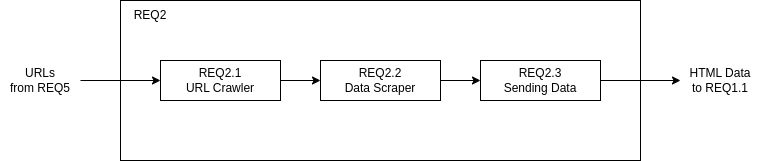
\includegraphics[width=\textwidth,keepaspectratio]{req2.png}\\

\textbf{REQ3:}

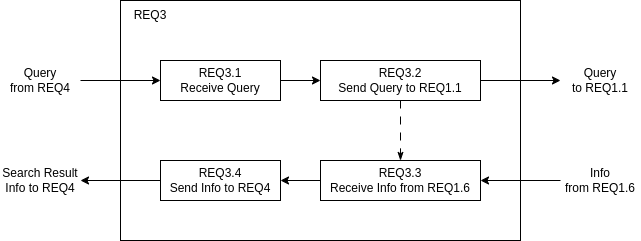
\includegraphics[width=\textwidth,keepaspectratio]{req3.png}\\

\textbf{REQ4:}

PLACEHOLDER FOR IMAGE ONCE REQ4 WRITTEN OUT\\

\textbf{REQ5:}

PLACEHOLDER FOR IMAGE ONCE REQ5 WRITTEN OUT\\

The following sections contain the detailed text descriptions of all the requirements in the project, grouped by top-level requirement, and sorted by requirement part number.

\subsection{REQ1: Search Engine Requirements}

\textit{This section will contain the detailed requirements for component 1: the search engine itself}



\subsection{REQ2: Backend Page Processing Requirements}


\textbf{\\REQ2.1:} The provided website url from \textbf{REQ5} is crawled  through upto a predefined limit.\par

\textbf{\\REQ2.2:} The crawled urls in \textbf{REQ2.1} are scraped for data.\par

\textbf{\\REQ2.3:} The data gathered in \textbf{REQ2.2} is sent to \textbf{REQ1.1} for processing.\par




\subsection{REQ3: Backend Query Processing Requirements}

\textbf{REQ3.1:}
\text{Receive user query from REQ4.\\} 
\textbf{\\REQ3.2:}
\text{call REQ1 with the input received in REQ3.1.\\}
\textbf{\\REQ3.3:}
\text{Receive pages with highlighting featuring the requested information from REQ1.\\} 
\textbf{\\REQ3.4:}
\text{Send the information received in REQ3.3 to REQ4 to be displayed to the user.}



\subsection{REQ4: Frontend Search Requirements}

\textbf{\\REQ4.1:} User has ability to enter a text input to search bar, which sends a request to \textbf{REQ3} and receives a response containing the indexed search results.\par

\textbf{\\REQ4.2:} The search results will be displayed on the results page and the user can select the desired result linking them to the designated URL for the respective result.\par



\subsection{REQ5: Frontend Page Add Requirements}

\textbf{\\REQ5.1:} Implement a user registration feature that requires a unique username and password. User will receive verification message and their respective data will be hashed and stored.\par

\textbf{\\REQ5.2:} Users have ability to request admin verification, which gives the capability of adding new pages to the search engine utilising the Backend Service from \textbf{REQ1.1}.\par


